\documentclass[a4paper,10pt]{article}
\usepackage[utf8]{inputenc}
\usepackage[spanish]{babel}
\usepackage[affil-it]{authblk}
\usepackage{enumerate}
\usepackage{graphicx}
\usepackage{hyperref}
\usepackage{amsmath}
\usepackage{amssymb}
\usepackage{cancel}
\usepackage[usenames, dvipsnames]{color}
\usepackage{tikz}
\usepackage{multimedia}
\usepackage{subcaption} %Multiple images
\usepackage{multicol} % Multiple columns
\usepackage{float}
\usepackage{cleveref}
\usepackage[margin=1.4in]{geometry}
\usepackage[labelfont=bf]{caption}
\usepackage[titletoc,toc,title]{appendix}
\usepackage{enumitem}
\usetikzlibrary{calc}
\numberwithin{equation}{section}

%Appendices in spanish
\renewcommand{\appendixname}{Ap\'endices}
\renewcommand{\appendixtocname}{Ap\'endices}
\renewcommand{\appendixpagename}{Ap\'endices}

%Zero delimiter
\newcommand{\zerodel}{.\kern-\nulldelimiterspace}

%Columns separation
\setlength{\columnsep}{1cm}

%Indentation
\setlength{\parindent}{0ex}

%Multiple References

\usepackage{xparse}
\ExplSyntaxOn
\NewDocumentCommand{\mref}{m}{\quinn_mref:n {#1}}
\seq_new:N \l_quinn_mref_seq
\cs_new:Npn \quinn_mref:n #1
 {
  \seq_set_split:Nnn \l_quinn_mref_seq { , } { #1 }
  \seq_pop_right:NN \l_quinn_mref_seq \l_tmpa_tl
  ( % print the left parenthesis
  \seq_map_inline:Nn \l_quinn_mref_seq
    { \ref{##1},\nobreakspace } % print the first references
  \exp_args:NV \ref \l_tmpa_tl 
  ) 
 }
\ExplSyntaxOff


%Boxes

\newcommand*{\boxcolor}{blue}
\makeatletter
\renewcommand{\boxed}[1]{\textcolor{\boxcolor}{%
\tikz[baseline={([yshift=-1ex]current bounding box.center)}] \node [rectangle, minimum width=1ex,rounded corners,draw] {\normalcolor\m@th$\displaystyle#1$};}}
 \makeatother

%Constantes
\newcommand{\euler}{\mathrm{e}}
\newcommand{\im}{i}

%Lemas, teoremas, definiciones y pruebas
\newcommand{\definicion}{\textbf{Definición: }}
\newcommand{\lema}{\textbf{Lema: }}
\newcommand{\teorema}{\textbf{Teorema: }}
\newcommand{\prueba}{\textbf{Prueba: }}


%opening
\title{Mecánica Clásica Tarea \# 7}
\author{Favio Vázquez\thanks{Correo: favio.vazquezp@gmail.com}}\affil{Instituto de Ciencias Nucleares. Universidad Nacional Autónoma de México.}
\date{}

\begin{document}

\makeatletter
\def\@maketitle{%
  \newpage
  \null
  \vskip 2em%
  \begin{center}%
  \let \footnote \thanks
    {\Large\bfseries \@title \par}%
    \vskip 1.5em%
    {\normalsize
      \lineskip .5em%
      \begin{tabular}[t]{c}%
        \@author
      \end{tabular}\par}%
    \vskip 1em%
    {\normalsize \@date}%
  \end{center}%
  \par
  \vskip 1.5em}
\makeatother

\maketitle

\section{Problema 1}

En presencia de la gravedad, dos discos uniformes de masa $m$ y radio $R$ unidos por 
un eje de longitud $l$ en torno al cual ambos giran libremente, descansan sobre un plano 
inclinado por un ángulo $\alpha$. Inicialmente se encuentran en reposo y el eje hace un ángulo 
$\beta$ con la dirección de máximo descenso. Si los discos ruedan sin resbalar determine 
las curvas que, sobre el plano, trazan los dos puntos de contacto entre los disco y el plano.

\vspace{.3cm}

\underline{Solución:} \vspace{.3cm}

Debido a la complejidad de este problema, y como en últimas la posición del eje 
está determinada por la posición de los discos, consideramos que podemos resolver 
el problema y determinar las curvas que traza el centro del eje, el cual representa
cómo se mueve el sistema sobre el plano, siguiendo a . Además para nuestra formulación, aunque 
exista el ángulo $\beta$ que hace el eje con la dirección de máximo descenso, nos será 
más útil el ángulo que hace el eje con el eje horizo tal que definiremos a continuación 
en el plano inclinado. Entonces, sean $XX'$ y $YY'$ un sistema de ejes perpendiculares 
sobre el plano inclinado, estando $YY'$ en dirección de máximo descenso. El centro 
$O$ del eje está caracterizado por las coordenadas $X$ e $Y$ en este sistema, con 
origen arbitrario $A$. Denotaremos por $\xi$ y $\xi'$ a los centros de los discos, y la 
distancia $l=\xi\xi'$. Debajo se encuentra una imagen ilustrativa del sistema físico,

\begin{figure}[H]
 \center
 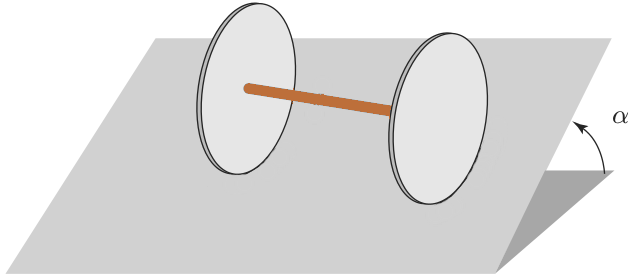
\includegraphics[scale=0.4]{problema1fig1}
 \caption{Representación esquemática del sistema de dos discos que ruedan sin resbalar.}
 \label{fig:problema1fig1}
\end{figure}

Para los discos, el eje puede considerarse como un eje de simetría, y entonces los 
momentos de inercia en el plano de los discos serán iguales $I_1 = I_2 = I$ y a lo 
largo de el eje $\xi\xi'$ será $I_3$. El eje hace un ángulo $\theta$ con la horizontal 
$XX'$. Denotaremos por $\theta$ y $\theta'1$ los ángulos que marcan los puntos de 
referencia de los puntos en la circunferencia de los discos con respecto a la línea 
normal al plano inclinado. Entonces con esas suposiciones y geometría que hemos 
planteado proponemos que podemos describir el sistema en términos de 5 coordenadas 
generalizadas $(X,Y,\theta,\phi,\phi')$. Debajo mostramos el sistema visto de arriba 
para una más fácil visualización de las coordenadas y de los ángulos que hemos 
planteado.

\begin{figure}[H]
 \center
 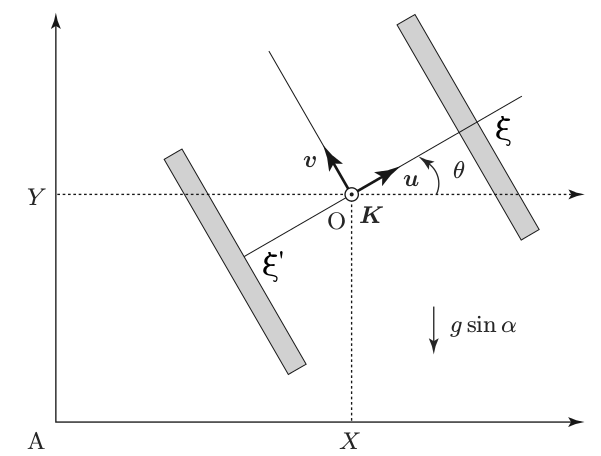
\includegraphics[scale=0.4]{problema1fig2}
 \caption{Geometría del sistema de ejes propuesto sobre el plano inclinado visto desde 
 arriba.}
 \label{fig:problema1fig2}
\end{figure}

Recordamos que el sistema está definido en el plano inclinado, con origen $A$, el eje 
horizontal es $AX$, el eje $AY$ está en la dirección de máximo descenso y $AZ$ es normal 
al plano. Las coordenadas del centro del eje, $O$, las denotaremos por $X$ y $Y$. Sea 
$\mathbf{K}$ el vector unitario normal al plano, $\mathbf{u}$ el vector unitario 
a lo largo de $\mathbf{O\xi}$ y $\mathbf{v}$ el vector unitario del plano perpendicular 
a $\mathbf{O\xi}$. Por esta construcción es fácil ver que $\mathbf{O\xi} = (l/2)\mathbf{u}$.
Debido a que también por construcción $\mathbf{A\xi} = \mathbf{AO} + \mathbf{O\xi}$ la 
velocidad del punto $\xi$ será $\mathbf{V}_\xi = \mathbf{V}_O + (l/2)\dot{\theta}\mathbf{v}$. 
Para obtener las cantidades relativas a $\xi'$ solo bastará con cambiar $l \rightarrow -l$ y 
$\phi \rightarrow \phi'$ a la cantidad relativa a $\xi$ lo cual simplificará 
bastante el trabajo.

\vspace{.3cm}

Debido a que el eje no tiene masa, solo los discos contribuyen a la energía 
cinética. Es fácil ver que el vector de rotación para el disco $\xi$ estará 
dado por $\mathbf{\omega} = \dot{\theta}\mathbf{K} + \dot{\phi}\mathbf{u}$. La 
energía cinética estará dada por la energía del centro de masa de la disco 
más la energía cinética de rotación,

\begin{equation}
 T_\xi = \frac{1}{2}\mathbf{V}_\xi^2 + T_\xi^{(rot)}.
\end{equation}

La energía rotacional se calcula simplemente utilizando $\mathbf{\omega}$ y
los momentos de inercia de los discos, $(T_\xi^{(rot)})_i = I_i(\mathbf{\omega}\cdot \mathbf{\omega})$, 
y ahora usando la expresión para $\mathbf{V}_\xi$ tenemos que 

\begin{equation}
 T_\xi = \frac{1}{2}m\left[\mathbf{V}_O^2 + (l^2/4)\dot{\theta}^2 +
 l\dot{\theta}\mathbf{v}\cdot\mathbf{V}_O \right]
 + \frac{1}{2}\left[ I\dot{\theta}^2 + I_3\dot{\phi}^2\right],
\end{equation}

y para $\xi'$

\begin{equation}
 T_{\xi'} = \frac{1}{2}m\left[\mathbf{V}_O^2 + (l^2/4)\dot{\theta}^2 
 - l\dot{\theta}\mathbf{v}\cdot\mathbf{V}_O \right]
 + \frac{1}{2}\left[ I\dot{\theta}^2 + I_3\dot{\phi}'^2\right].
\end{equation}

Ahora debido a que $\mathbf{V}_O^2 = \dot{X}^2 + \dot{Y}^2$ por la 
construcción que hemos hecho, y sumando las expresiones de las energías 
cinéticas para ambos discos tenemos que,

\begin{align*}
 T &= \frac{1}{2}m\left[(\dot{X}^2 + \dot{Y}^2) + (l^2/4)\dot{\theta}^2 +
 l\dot{\theta}\mathbf{v}\cdot\mathbf{V}_O \right]
 + \frac{1}{2}\left[ I\dot{\theta}^2 + I_3\dot{\phi}^2\right] \\
 %
 &+ \frac{1}{2}m\left[(\dot{X}^2 + \dot{Y}^2) + (l^2/4)\dot{\theta}^2 
 - l\dot{\theta}\mathbf{v}\cdot\mathbf{V}_O \right]
 + \frac{1}{2}\left[ I\dot{\theta}^2 + I_3\dot{\phi}'^2\right], \\
 %
   &= \frac{1}{2}m(\dot{X}^2 + \dot{Y}^2) + \frac{1}{2}m(l^2/4)\dot{\theta}^2 +
      \cancel{\frac{1}{2}ml\dot{\theta}\mathbf{v}\cdot\mathbf{V}_O}
      + \frac{1}{2}I\dot{\theta}^2 + \frac{1}{2}I_3\dot{\phi}^2 \\
  %
  &+ \frac{1}{2}m(\dot{X}^2 + \dot{Y}^2) + \frac{1}{2}m(l^2/4)\dot{\theta}^2 -
      \cancel{\frac{1}{2}ml\dot{\theta}\mathbf{v}\cdot\mathbf{V}_O}
      + \frac{1}{2}I\dot{\theta}^2 + \frac{1}{2}I_3\dot{\phi}'^2,
  %
\end{align*}

\begin{equation}
 \therefore T = m\left(\dot{X}^2 + \dot{Y}^2\right)  
 +\left( I + \frac{1}{4}ml^2 \right) \dot{\theta}^2 
 + \frac{1}{2}I_3 \left(\dot{\phi}^2 + \dot{\phi}'^2\right).
\end{equation}

Veremos que escribir las aceleraciones generalizadas nos será muy útil
para resolver este problema ya que lo haremos utilizando el método de 
los multiplicadores indeterminados de Lagrange. Recordando la expresión
para las aceleraciones generalizadas 

\begin{equation}
 A_i(q,\dot{q},\ddot{q},t) = \frac{d}{dt}\frac{\partial T(q,\dot{q},t)}{\partial\dot{q^i}}
 + \frac{\partial T(q,\dot{q},t)}{\partial q^i},
\end{equation}

tenemos entonces que,

\begin{align}
 A_X &= 2m\ddot{X}, \\
 A_Y &= 2m\ddot{Y}, \\
 A_\theta &= 2 \left( I + \frac{1}{4}ml^2 \right) \ddot{\theta}, \\
 A_\phi &= I_3\ddot{\phi}, \\
 A_{\phi'} &= I_3\ddot{\phi}''.
\end{align}

Necesitamos ahora expresar las condiciones para rodar sin resbalar. Sea 
$\zeta$ el punto de contacto del disco $\xi$con el plano; la condición que 
requerimos es que $\mathbf{V}_\zeta = 0$. Pero sabemos que para $\xi$, 
el vector de rotación instantánea en $\zeta$ puede escribirse como 

\begin{equation}
 \mathbf{V}_\zeta = \mathbf{V}_\xi + \mathbf{\omega}\times \mathbf{\xi\zeta} = 0.
\end{equation}

Esta condición nos dará dos condiciones escalares, lo mismo para 
el disco $\xi'$ que en el punto $\zeta'$ debe cumplirse que 

\begin{equation}
 \mathbf{V}_\zeta' = \mathbf{V}_\xi' + \mathbf{\omega}\times \mathbf{\xi'\zeta'} = 0.
\end{equation}

De estas cuatro condiciones (utilizando la figura \mref{fig:problema1fig2} y la ecuación para $\mathbf{V}_\xi$), 
dos son idénticas, y tenemos entonces tres ecuaciones de constricción,

\begin{align}
 \dot{X}\cos{\theta} + \dot{Y}\sen{\theta} = 0, \\
 \dot{Y}\cos{\theta} - \dot{X}\sen{\theta} + \frac{1}{2}l\dot{\theta} + R\dot{\phi} = 0, \\
 \dot{Y}\cos{\theta} - \dot{X}\sen{\theta} - \frac{1}{2}l\dot{\theta} + R\dot{\phi}' = 0,
\end{align}

Podemos escribir estas ecuaciones de una forma más informativa, haciendo 
un poco de álgebra, como

\begin{align}
\label{eq:discosConstri1}
 2\dot{X} - R (\dot{\phi} + \dot{\phi}')\sen{\theta} = 0, \\
\label{eq:discosConstri2}
 2\dot{Y} + R (\dot{\phi} + \dot{\phi}')\cos{\theta} = 0, \\
\label{eq:discosConstri3}
 l\dot{\theta} + R (\dot{\phi} - \dot{\phi}') = 0.
\end{align}

De estas constricciones, solo \mref{eq:discosConstri3} es holonómica, 
en cambio \mref{eq:discosConstri1} y \mref{eq:discosConstri2} son no holonómicas. 
Estas construcciones representan las constricciones requeridas para rodar 
sin resbalar. 

\vspace{.3cm}

Debido a que los puntos de aplicación para las fuerzas de reacción 
debidos al plano no se desplazan durante un desplazamiento virtual, 
por la condición de rodar sin resbalar, estas fuerzas de reacción no 
implican fuerzas generalizadas. El único trabajo virtual que no 
se hace cero es debido al peso. Podemos calcularla con un desplazamiento 
virtual del centro de masa $O$. Es fácil ver que 

\begin{equation}
 \delta W = - 2mg \delta z_O = -2mg\sen{\alpha}\delta Y,
\end{equation}

entonces la única fuerza generalizada que no se hace cero es 

\begin{equation}
 Q_Y = -2mg\sen{\alpha}.
\end{equation}

Ahora recordando la expresión para el formalismo de los multiplicadores 
indeterminados de Lagrange tenemos que, utilizando las expresiones 
para las aceleraciones generalizadas,

\begin{align}
 m\ddot{X} = \lambda_1, \\
 m\ddot{Y} = - mg\sen{\alpha} + \lambda_2, \\
 2\left( I + \frac{1}{4}ml^2\right) \ddot{\theta} = l\lambda_3, \\
 I_3\ddot{\phi} = -\lambda_1 R\sen{\theta} + \lambda_2 R\cos{\theta} + R\lambda_3, \\
 I_3\ddot{\phi}' = -\lambda_1 R\sen{\theta} + \lambda_2 R\cos{\theta} - R\lambda_3.
\end{align}


TERMINAR.


\section{Problema 2}

Un sistema consiste de una partícula de masa $m$ en el espacio físico y tiene una 
lagrangiana

$$
L = \frac{1}{2}m(\mathbf{\dot{r}} \cdot \mathbf{\dot{r}}) - V(\mathbf{r}).
$$

La partícula puede describir una trayectoria entre dos puntos $A$ y $B$ en un tiempo 
$t_{AB}$. Demuestre que una partícula de masa $M$ sujeta al mismo potencial podrá 
describir la misma trayectoria entre los puntos $A$ y $B$, pero que el tiempo que 
tardaría sería distinto. Calcule ese tiempo.

\vspace{.3cm}

\underline{Solución:} \vspace{.3cm}

Debido a que la lagrangiana no depende del tiempo y la energía potencial 
es una función homogénea cuadrática de las velocidades, se conserva la cantidad 
de Jacobi y esta es igual a la energía total del sistema, por lo tanto 
podemos escribir

\begin{equation}
 E = T + V = \frac{1}{2}m\dot{r}^2 + V,
\end{equation}

de esta ecuación podemos obtener el tiempo $t_{AB}$ que le toma a la primera 
partícula describir la trayectoria entre $AB$ como

\begin{equation}
 t_{AB} = \frac{\sqrt{m}}{\sqrt{2}} \int_A^B \frac{dr}{\sqrt{E - V}}.
 \label{eq:tiempo1}
\end{equation}

Por otra parte para la segunda partícula tendremos que

\begin{equation}
 E = \frac{1}{2}M\dot{r}^2 + V,
\end{equation}

por lo que el tiempo $\tau_{AB}$ que le toma a la segunda 
partícula describir la trayectoria entre $AB$ lo podemos escribir como

\begin{equation}
 t_{AB} = \frac{\sqrt{M}}{\sqrt{2}} \int_A^B \frac{dr}{\sqrt{E - V}}.
 \label{eq:tiempo2}
\end{equation}

Ahora dividiendo \mref{eq:tiempo1} entre \mref{eq:tiempo2} obtenemos que 

\begin{equation}
 \frac{t_{AB}}{\tau_{AB}} = \frac{\sqrt{m}/\sqrt{2}}{\sqrt{M}/\sqrt{2}} 
 \frac{\int_A^B \frac{dr}{\sqrt{E - V}}}{\int_A^B \frac{dr}{\sqrt{E - V}}}
\end{equation}

\begin{equation}
 \frac{t_{AB}}{\tau_{AB}} = \left(\frac{m}{M}\right)^{\frac{1}{2}}
\end{equation}

\begin{equation}
 \boxed{\therefore t_{AB} = \left(\frac{m}{M}\right)^{\frac{1}{2}}\tau_{AB}}
\end{equation}

Por lo tanto hemos demostrado que  partícula de masa M sujeta al mismo potencial 
describirá la misma trayectoria entre los puntos A y B, pero que el tiempo que tardaría sería distinto. Claramente cuando 
$m = M$ el tiempo será el mismo.





\section{Problema 3}

Una funcional $f(y)$ $(y(t) \in \mathbb{R}^n)$ se define por 

$$
f(y) = \int_{t_{i}}^{t_{f}} F(y,\dot{y},\ddot{y},y)dt.
$$

Encuentre las condiciones o ecuaciones que debe cumplir la curva $y$ para que $f$ sea
extremal cuando fijamos $y(t_i) = y_i$, $y(t_f)=y_f$, $\dot{y}(t_i) = v_i$ y
$\dot{y}(t_f) = v_f$.

\vspace{.3cm}

\underline{Solución:} \vspace{.3cm}

Comencemos calculando la diferencial de la funcional dada, claramente esta debe ser 
diferenciable para poder cumplirse lo que demostraremos en este problema. Usando 
el hecho de 

\begin{equation}
 F(c+h) - F(c) = DF_c[h]+O(|h|^2),
 \label{eq:diferencialFuncional1}
\end{equation}

donde $c$ y $h$ son curvas, y $Df_c$ es una funcional lineal, a la cual se le llama 
la diferencial de la funcional $f$ valuada en la curva $c$, tenemos entonces que, 
donde recordamos que $y = y(t)$, $\dot{y} = \dot{y}(t)$,$\ddot{y} = \ddot{y}(t)$ y $h=h(t)$, 
$\dot{h}=\dot{h}(t)$, $\ddot{h}=\ddot{h}(t)$

\begin{align}
\begin{split}
 f(y+h) - f(y) &= \int_{t_{i}}^{t_{f}} F(y+h,\dot{y}+ \dot{h}, \ddot{y} + \ddot{h}, t)dt -
 \int_{t_{i}}^{t_{f}} F(y,\dot{y},\ddot{y},y)dt, \\
	       &= \int_{t_{i}}^{t_{f}} \left[ F(y+h,\dot{y}+ \dot{h}, \ddot{y} + \ddot{h}, t)
	       -F(y,\dot{y},\ddot{y},y) \right]dt.
 \end{split}
\end{align}

Ahora, como $F$ es una función diferenciable de $\mathbb{R}^{n+n+n+1}$ en $R$ podemos 
escribir, utilizando \mref{eq:diferencialFuncional1}

\begin{equation}
 f(y+h) - f(y) =  \int_{t_{i}}^{t_{f}} \left\{DF_y[h,\dot{h},\ddot{h},t] + O(|h|^2) \right\}dt
\end{equation}

Luego,

\begin{align*}
 f(y+h) - f(y) = \int_{t_{i}}^{t_{f}} \left[ \left\zerodel \sum_{i=1}^n  \left( \frac{\partial F}{\partial y_i}h_i + 
 \frac{\partial F}{\partial \dot{y}_i}\dot{h}_i + \frac{\partial F}{\partial \ddot{y}_i}\ddot{h}_i\right)\right|_{y} 
 + O(|h|^2) \right]dt, \\
%  
	      = \sum_{i=1}^n \left[\int_{t_{i}}^{t_{f}}\left\zerodel\frac{\partial F}{\partial y_i}\right|_y h_i dt  
	      + \int_{t_{i}}^{t_{f}} \left\zerodel\frac{\partial F}{\partial \dot{y}_i}\right|_y \dot{h}_i dt
	       + \int_{t_{i}}^{t_{f}} \left\zerodel\frac{\partial F}{\partial \ddot{y}_i}\right|_y \ddot{h}_i dt\right] 
	       +  \int_{t_{i}}^{t_{f}} O(|h|^2)dt
 %
\end{align*}

Integrando por parte el segundo y el primer término tenemos que

\begin{equation}
  \int_{t_{i}}^{t_{f}} \left\zerodel\frac{\partial F}{\partial \dot{y}_i}\right|_y \dot{h}_i dt = 
  - \int_{t_{i}}^{t_{f}} \frac{d}{dt}\left(\left\zerodel\frac{\partial F}{\partial \dot{y}}\right)\right|_y h_i dt + 
  \left\zerodel\frac{\partial F}{\partial \dot{y}}\right|_y \left\zerodel h_i\right|_{t_{i}}^{t_{f}},
\end{equation}

y

\begin{equation}
  \int_{t_{i}}^{t_{f}} \left\zerodel\frac{\partial F}{\partial \ddot{y}_i}\right|_y \ddot{h}_i dt = 
  - \int_{t_{i}}^{t_{f}} \frac{d}{dt}\left(\left\zerodel\frac{\partial F}{\partial \ddot{y}}\right)\right|_y \dot{h}_i dt + 
  \left\zerodel\frac{\partial F}{\partial \ddot{y}}\right|_y \left\zerodel \dot{h}_i\right|_{t_{i}}^{t_{f}},
\end{equation}

Entonces tenemos que,

\begin{align}
 \begin{split}
  f(y+h) - f(y) =  &\sum_{i=1}^n \left[\int_{t_{i}}^{t_{f}}\left\zerodel\frac{\partial F}{\partial y_i}\right|_y h_i dt 
   - \int_{t_{i}}^{t_{f}} \frac{d}{dt}\left(\left\zerodel\frac{\partial F}{\partial \dot{y}}\right)\right|_y h_i dt + 
  \left\zerodel\frac{\partial F}{\partial \dot{y}}\right|_y \left\zerodel h_i\right|_{t_{i}}^{t_{f}}\right\zerodel \\
  %
  &- \left\zerodel\int_{t_{i}}^{t_{f}} \frac{d}{dt}\left(\left\zerodel\frac{\partial F}{\partial \ddot{y}}\right)\right|_y \dot{h}_i dt + 
  \left\zerodel\frac{\partial F}{\partial \ddot{y}}\right|_y \left\zerodel \dot{h}_i\right|_{t_{i}}^{t_{f}}\right]
  +  \int_{t_{i}}^{t_{f}} O(|h|^2)dt \\
  %
  &= \sum_{i=1}^n\left[\int_{t_{i}}^{t_{f}}\left\zerodel\frac{\partial F}{\partial y_i}\right|_y h_i dt 
   - \int_{t_{i}}^{t_{f}} \frac{d}{dt}\left(\left\zerodel\frac{\partial F}{\partial \dot{y}}\right)\right|_y h_i dt + 
  \left\zerodel\frac{\partial F}{\partial \dot{y}}\right|_y \left\zerodel h_i\right|_{t_{i}}^{t_{f}}\right\zerodel \\
  %
  &-\left\zerodel \int_{t_{i}}^{t_{f}} \frac{d^2}{dt^2}\left(\left\zerodel\frac{\partial F}{\partial \ddot{y}}\right)\right|_y h_i dt + 
  \left\zerodel\frac{\partial F}{\partial \ddot{y}}\right|_y \left\zerodel \dot{h}_i\right|_{t_{i}}^{t_{f}}\right]
  +  \int_{t_{i}}^{t_{f}} O(|h|^2)dt
  %
 \end{split}
\end{align}

Tenemos entonces que 

\begin{align*}
 f(y+h) - f(y) &= \sum_{i=1}^n \int_{t_{i}}^{t_{f}} \left[\frac{\partial F}{\partial y_i}  - 
 \frac{d}{dt}\frac{\partial F}{\partial \dot{y}}  
 - \frac{d^2}{dt^2}\frac{\partial F}{\partial \ddot{y}} \right]_y h_i dt \\
 &+\sum_{i=1}^n \left\zerodel \left\zerodel\frac{\partial F}{\partial \dot{y}}\right|_y h_i\right|_{t_{i}}^{t_{f}}
 + \sum_{i=1}^n \left\zerodel \left\zerodel\frac{\partial F}{\partial \ddot{y}}\right|_y\dot{h}_i\right|_{t_{i}}^{t_{f}}
 + \int_{t_{i}}^{t_{f}} O(|h|^2)dt
\end{align*}

Tenemos entonces que la diferencial está dada por

\begin{align}
\begin{split}
 DF_c[h] &=  \sum_{i=1}^n \int_{t_{i}}^{t_{f}} \left[\frac{\partial F}{\partial y_i}  - 
 \frac{d}{dt}\frac{\partial F}{\partial \dot{y}}  
 - \frac{d^2}{dt^2}\frac{\partial F}{\partial \ddot{y}} \right]_y h_i dt \\
 &+\sum_{i=1}^n \left\zerodel \left\zerodel\frac{\partial F}{\partial \dot{y}}\right|_y h_i\right|_{t_{i}}^{t_{f}}
 + \sum_{i=1}^n \left\zerodel \left\zerodel\frac{\partial F}{\partial \ddot{y}}\right|_y\dot{h}_i\right|_{t_{i}}^{t_{f}}
 \end{split}
 \label{eq:diferencialFuncional2}
\end{align}


Para resolver este problema, limitamos las posibles curvas a aquellas que 
para pasan por puntos fijos, y que cumplen con las condiciones del enunciado, con lo 
cual vemos que la variación de $h_i$ y $\dot{h}_i$ es cero evaluada entre $t_i$ y $t_f$, 
haciendo cero a los dos últimos términos de \mref{eq:diferencialFuncional2}, y entonces 
como el resto de las cantidades dentro del primer término de \mref{eq:diferencialFuncional2}
son independientes de $h(t)$, para que se cumpla que la curva $y$ para que $f$ sea 
extremal debe cumplirse que 

\begin{equation}
\boxed{\frac{\partial F}{\partial y_i}  - 
 \frac{d}{dt}\frac{\partial F}{\partial \dot{y}}  
 - \frac{d^2}{dt^2}\frac{\partial F}{\partial \ddot{y}} = 0.}
 \label{eq:condicionExtremal}
\end{equation}

Decimos entonces que la funcional $f$, y dentro del espacio de las curvas que pasan 
por un punto específico para $t=t_0$ y por otro para $t=t_1$, las curvas para que la 
funcional tiene una extremal están dadas por las ecuaciones \mref{eq:condicionExtremal}.



\section{Problema 4}

Demuestre que la formulación lagrangiana de la mecánica es invariante ante el grupo 
de Galileo.

\vspace{.3cm}

\underline{Solución:} \vspace{.3cm}

\textbf{Nota}: Luego de una charla con el profesor nos comentó que solo teníamos que probar 
la invariancia ante los ``boosts'', es decir las transformaciones cinemáticas..

\noindent\rule[0.5ex]{\linewidth}{1pt}

El marco inercial con el cual podemos describir un sistema mecánico no es único, de hecho 
existe un número infinito de marcos inerciales. Sea $S$ un marco inercial. Puede probarse 
\cite{tong} que hay $10$ transformaciones independientes $S\rightarrow S$ tales que 
$S'$ también sea un marco inercial. Estas son:

\begin{itemize}
 \item 3 Rotaciones: $\mathbf{r}' = O\mathbf{r}$ donde $O$ es una matriz ortogonal $3\times 3$.
 \item 3 Traslaciones: $\mathbf{r}' = \mathbf{r} + \mathbf{c}$ para un vector constante $\mathbf{c}$.
 \item 3 ``boosts'' (impulsos): $\mathbf{r}' = \mathbf{r} + \mathbf{v}t$ para una velocidad constante 
 $\mathbf{v}$.
 \item 1 Traslación temporal: $t' = t+c$ para una constante real $c$.
\end{itemize}

Estas transformaciones conforman el grupo de Galileo, el cual es un grupo de 10 parámetros. 
Como hemos dicho solo probaremos la invariancia ante los ``boosts''. Recordemos que podemos 
escribir la lagrangiana de la forma

\begin{equation}
 L = T-V = \frac{1}{2}m(\mathbf{v}\cdot \mathbf{v}) - V,
 \label{eq:lagrangianaGalileo1}
\end{equation}

y sea una transformación de la forma

\begin{equation}
 \mathbf{r}' = \mathbf{r} + \mathbf{v_0}t, \qquad \mathbf{v}' = \mathbf{v} + \mathbf{v_0}.
\label{eq:boost1}
\end{equation}

Entonces tenemos que la lagrangiana para el sistema $S'$ estará dada por

\begin{equation}
 L' = \frac{1}{2}m(\mathbf{v}'\cdot \mathbf{v}') - V,
\end{equation}

pero por \mref{eq:boost1} 

\begin{align*}
 L'&= \frac{1}{2}m[(\mathbf{v} + \mathbf{v_0})\cdot(\mathbf{v} + \mathbf{v_0})] - V, \\
   &= \frac{1}{2}m(\mathbf{v}\cdot \mathbf{v} + 2\mathbf{v}\cdot \mathbf{v}_0 + \mathbf{v}_0\cdot \mathbf{v}_0) - V, \\
   &= \frac{1}{2}m(\mathbf{v}\cdot \mathbf{v}) - V + \frac{1}{2}m(2\mathbf{v}\cdot \mathbf{v}_0) + \frac{1}{2}m(\mathbf{v}_0\cdot \mathbf{v}_0),
\end{align*}

pero por \mref{eq:lagrangianaGalileo1} tenemos que 

\begin{equation}
 L' = L + \frac{1}{2}m\mathbf{v}_0(2\mathbf{v}+\mathbf{v}_0)
 \label{eq:lagrangianaGalileo2}
\end{equation}

Ahora debido a que\footnote{Recordar que $\mathbf{v}_0$ es constante.}

\begin{equation}
 \frac{1}{2}m\mathbf{v}_0(2\mathbf{v}+\mathbf{v}_0) = \frac{d}{dt}\left[\frac{1}{2}m\mathbf{v}_0(2\mathbf{r}+\mathbf{v}_0t)\right]
 = \frac{d}{dt}\phi,
\end{equation}

donde $\phi \equiv \frac{1}{2}m\mathbf{v}_0(2\mathbf{r}+\mathbf{v}_0t)$. Entonces 
\mref{eq:lagrangianaGalileo2} se transforma en 

\begin{equation}
 \boxed{L' = L + \frac{d}{dt}\phi}
\end{equation}

Vemos entonces que debido a que como ya se ha demostrado en tareas anteriores, dos lagrangianas 
diferentes resultarán en ecuaciones de movimiento idénticas si difieren solamente 
por una función de las coordenadas y el tiempo. Con lo cual hemos demostrado que 
la formulación lagrangiana es invariante ante el grupo de Galileo, particularmente 
queríamos probar que era invariante ante transformaciones del tipo ``boost''.

\section{Problema 5}

Demuestre, con toda formalidad y usando el teorema de Noether, que la lagrangiana 
de una partícula libre en tres dimensiones es invariante ante el grupo de rotaciones 
$SO(3)$ y que por ello se conserva el vector de impulso angular.

\vspace{.3cm}

\underline{Solución:} \vspace{.3cm}

Comenzaremos con una breve digresión de teoría de grupos necesaria para poder dar una 
demostración completa y formal del enunciado de este problema. Utilizando principalmente 
el contenido básico de \cite{tung}. Además haremos una breve descripción del teorema 
de Noether para simetrías continuas tomado en gran parte de \cite{kleinert}.

\vspace{.3cm}

\definicion (Grupo): Se dice que un conjunto $\{G:a,b,c,\dots\}$ forma un \emph{grupo}
si existe una operación $\cdot$, llamada la \emph{multiplicación de grupo}, que asocia 
cualquier par de elementos (ordenados) dado $a,b \in G$ con un producto bien definido 
$a\cdot b$ que también es un elemento de $G$, tal que se satisfacen las siguientes 
condiciones 

\begin{enumerate}[label=(\alph*)]
 \item La operación $\cdot$ es \emph{asociativa}, i.e. $a\cdot (b\cdot c) = (a\cdot b)\cdot c$ 
 para todo $a,b,c \in G$,
 \item Entre los elementos de $G$, existe un elemento $e$, llamado la identidad, que 
 tiene la propiedad de que $a\cdot e = a$ para todo $a \in G$,
 \item Para cada $a \in G$, existe un elemento $a^{-1} \in G$, llamado la inversa 
 de $a$ que tiene la propiedad de que $a\cdot a^{-1} = e$.
\end{enumerate}

\definicion (Grupo Abeliano): Un \emph{grupo abeliano} $G$ es aquel en que la multiplicación
de grupo es conmutativa, i.e. $a\cdot b = b\cdot a$ para todo $a,b \in G$.

\vspace{.3cm}

De la definición anterior diremos que un grupo puede ser abeliano o no-abeliano.

\vspace{.3cm}

\definicion (Orden): El \emph{orden} de un grupo es el número de elementos del grupo 
(si es finito). 

\vspace{.3cm}

\definicion (Grupo continuo): Los \emph{grupos continuos} consisten en grupos de 
elementos etiquetados por una o más variables continuas, i.e. $(a_1,a_2,\dots,a_r)$, 
donde cada variable tiene un rango bien definido.

\vspace{.3cm}

Claramente todos los grupos continuos tienen un número infinito de elementos, aunque 
puede probarse que no todos los grupos infinitos son continuos. La teoría matemática 
general de grupos continuos es usualmente llamada la teoría de grupos de Lie. Simplificando,
podemos decir que un \emph{grupo de Lie} es un grupo infinito cuyos elementos pueden 
ser parametrizados suave y analíticamente; la formulación precisa de los grupos de 
Lie requiere un trato considerable ya que envuelve nociones de topología y geometría 
diferencial, las cuales salen del marco de desarrollo de este problema.

\vspace{.3cm}

Pasemos ahora a estudiar brevemente el grupo que nos interesa para solucionar este 
problema, \textbf{SO(3)}, el grupo continuo no-abeliano más útil \cite{tung}.

\vspace{.3cm}

\definicion (Grupo \textbf{SO(3)}): El \emph{grupo \textbf{SO(3)}} consiste en todas 
las transformaciones lineales continuas en el espacio euclideano tridimensional 
que dejan la longitud de los vectores coordenados invariantes. 

\vspace{.3cm}

Consideremos un sistema de coordenadas Cartesiano especificado por los vectores 
ortonormales $\hat{\mathbf{e}}_i$, $i = 1,2,3$. Bajo la rotación,

\begin{equation}
 \hat{\mathbf{e}}_i \xrightarrow{\mathbf{R}} \hat{\mathbf{e}}'_i = \hat{\mathbf{e}}_j R^j_i,
\end{equation}

donde $R^j_i$ son elementos de matrices rotacionales $3\times 3$. Sea $\mathbf{x}$ un 
vector arbitrario, $\mathbf{x} = \hat{\mathbf{e}}_i x^i$, entonces 
$\mathbf{x} \rightarrow \mathbf{x}'$ bajo la rotación $\mathbf{R}$ tal que

\begin{equation}
 x'^{i} = R^i_j x^j. 
\end{equation}

El requerimiento que $|\mathbf{x}| = |\mathbf{x}'|$, o $x_i x^j = x'_i x'^{j}$, resulta en 

\begin{equation}
 \mathbf{R}\mathbf{R}^T = \mathbf{R}^T\mathbf{R} = \mathbf{E},
 \label{eq:identidadSO31}
\end{equation}

donde $\mathbf{E}$ es la matriz identidad, para todas las matrices rotacionales. Las 
matrices reales que satisfacen esta condición tienen determinantes igual a $\pm 1$. Debido 
a que todas las rotaciones físicas pueden ser alcanzadas continuamente de la 
la transformación idéntica (ángulo cero de rotación), y debido a que el determinante 
de esta es $+1$, entonces todas las matrices de rotación deben tener determinante $+1$. Entonces 
en adición a la ecuación \mref{eq:identidadSO31}, las matrices $\mathbf{R}$ están restringidas 
por la condición

\begin{equation}
 \text{det } \mathbf{R} = 1.
 \label{eq:unoSO31}
\end{equation}

Ambas condiciones para la matriz rotacional $\mathbf{R}$ pueden ser expresadas 
en términos de \emph{tensores invariantes}. En particular la ecuación \mref{eq:identidadSO31} 
puede escribirse como

\begin{equation}
 R^i_k R^j_l \delta^{kl} = \delta^{ij}, 
 \label{eq:identidadSO32}
\end{equation}

que expresa la invariancia del tensor de segundo orden $\delta^{kl}$ (conocido como
la delta de Kronecker) bajo rotaciones. De forma similar, la ecuación \mref{eq:unoSO31} 
puede escribirse como

\begin{equation}
 R^i_l R^k_m R^k_n \epsilon^{lmn} = \epsilon^{ijk},
 \label{eq:unoSO32}
\end{equation}

donde $\epsilon^{ijk}$ es el tensor unitario de tercer orden totalmente antisimétrico (conocido 
como el tensor de Levi-Civita). Cuando $(i,j,k) = (1,2,3)$, el lado izquierdo 
de \mref{eq:unoSO32} es simplemente la determinante; y esta ecuación coincide con 
\mref{eq:unoSO31}. Para otros valores de $(i,j,k)$, la identidad resulta de la naturaleza 
totalmente antisimétrica de los ambos lados de la ecuación. Esta identidad establece 
el hecho de que $e^{lmn}$ es invariante ante rotaciones. 

\vspace{.3cm}

Pasemos ahora a un breve estudio de simetrías continuas, leyes de conservación y 
el teorema de Noether. Consideremos a sistema mecánico simple con una acción 
generadora

\begin{equation}
 \mathcal{A} = \int_{t_{a}}^{t_{b}} L(q(t),\dot{q}(t),t)dt.
 \label{eq:noet1}
\end{equation}

Supongamos que $\mathcal{A}$ es invariante bajo un conjunto continuo de transformaciones 
de las variables dinámicas:

\begin{equation}
 q(t) \rightarrow q'(t) = f(q(t),\dot{q}(t)),
 \label{eq:noet2}
\end{equation}

donde $f(q(t),\dot{q}(t))$ es alguna funcional de $q(t)$. Estas transformaciones 
son llamadas transformaciones de simetría. Si la acción se somete a dos transformaciones 
de simetría sucesivas, el resultado es de nuevo una transformación de simetría. Entonces, 
las transformaciones de simetría forman el llamado \emph{grupo de simetría} del sistema. 
Para una transformación infinitesimal \mref{eq:noet2}, la diferencia 

\begin{equation}
 \delta_s q(t) \equiv q'(t) - q(t),
 \label{eq:noet3}
\end{equation}

es llamada una \emph{variación de simetría}. Tiene la forma general 

\begin{equation}
 \delta_s = \epsilon \xi((q(t),\dot{q}(t),t)).
 \label{eq:noet4}
\end{equation}

Si calculamos el cambio de la acción bajo la acción de simetría \mref{eq:noet4}, utilizando
la regla de la cadena para la diferenciación, la integración por partes y el hecho
de que deben cumplirse las ecuaciones de Lagrange para las trayectorias de $q(t)$, obtendremos 
que la cantidad 

\begin{equation}
 I(t) = \frac{\partial L}{\partial \dot{q}}\xi(q,\dot{q},t),
 \label{eq:noet5}
\end{equation}

es la misma para los tiempo $t=t_a$ y $t=t_b$. Debido a que $t_b$ es arbitrario, 
$I(t)$ es independiente del tiempo, i.e., satisface

\begin{equation}
 I(T) \equiv I.
 \label{eq:noet6}
\end{equation}

Entonces $I$ es una cantidad conservada, una constante de movimiento. El lado derecho 
de \mref{eq:noet5} es llamada la \emph{carga de Noether}, y lo que hemos enunciado en 
este breve estudio es el conocido \emph{teorema de Noether}.

\vspace{.3cm}

Consideremos ahora la lagrangiana para una partícula libre en el espacio tridimensional

\begin{equation}
 L = L(q^i(t),\dot{q}^i(t),t).
\end{equation}

Bajo el grupo de rotaciones \textbf{SO(3)}, las coordenadas $q^i$ cambian a

\begin{equation}
 q'^i = R^i_j q^j,
\end{equation}

donde $ R^i_j$ es de la forma que hemos definido arriba. Infinitesimalmente, podemos 
escribir esto como

\begin{equation}
 R^i_j = \delta^i_j - \omega_l \epsilon_{kij},
\end{equation}

donde $\mathbf{\omega}$ es un vector de rotación infinitesimal. La correspondiente 
rotación del camino de la partícula es 

\begin{equation}
 \delta_s q^i(t) = q'^i(t) - q^i(t) = - \omega^k\epsilon_{kij}q^j.
\end{equation}

Es útil en este punto introducir el tensor de rotación antisimétrico infinitesimal 

\begin{equation}
 \omega_{ij} \equiv \omega_k \epsilon{kij},
\end{equation}

y en términos de este tenemos que

\begin{equation}
 \delta_s q^i = -\omega_{ij}q^j.
\end{equation}
 
Podemos ahora escribir el cambio en la lagrangiana bajo $\delta q^i$,

\begin{align}
\begin{split}
 \delta_s L &= L(q'^i(t),\dot{q}'^i,t) - L(q^i(t),\dot{q}^i,t), \\
	    &= \frac{\partial L}{\partial q^i}\delta_s q^i + \frac{\partial L}{\partial \dot{q}^i}\delta_s \dot{q}^i,
 \end{split}
\end{align}

como

\begin{equation}
 \delta_s L = - \left(\frac{\partial L}{\partial q^i}q^i +  
  \frac{\partial L}{\partial \dot{q}^i}\dot{q}^i\right)\omega_{ij} = 0.
\end{equation}

Si la lagrangiana depende solamente de invariantes de rotación, y sus potencias, entonces 
el lado derecho se hace cero debido a la antisimetría de $\omega_ij$. Esto asegura 
simetría rotacional. Podemos ahora hacer otra variación simétrica de la lagrangiana 
usando la regla de la cadena, usando las ecuaciones de Lagrange, 

\begin{align}
 \begin{split}
  \delta_s L &= \left( \frac{\partial L}{\partial q^i} - \frac{d}{dt} \frac{\partial L}{\partial \dot{q}^i} 
  \right)\delta_s q^i + \frac{d}{dt}\left( \frac{\partial L}{\partial \dot{q}^i}\delta_s q^i \right), \\
  %
	   &= -\frac{d}{dt}\left( \frac{\partial L}{\partial \dot{q}^i} \right)\omega_{ij} 
	   = \frac{1}{2}\frac{d}{dt}\left(q_i  \frac{\partial L}{\partial \dot{q}^i}  
	   -  q_j\frac{\partial L}{\partial \dot{q}^j}\right)\omega_{ij}.
 \end{split}
\end{align}

El lado derecho de esta ecuación nos da la carga de Noether conservada de la forma 
\mref{eq:noet5}, una para cada par antisimétrico $i,j$:

\begin{equation}
 \boxed{K^{ij} = x^i\frac{\partial L}{\partial \dot{q}^j} - x^j\frac{\partial L}{\partial \dot{q}^i} 
 = x^i p^j - x^j p^i.}
\end{equation}

Estas son las componentes antisimétricas del momentum angular $K^{ij}$. Si trabajamos 
con la forma vectorial original para los ángulos de rotación $\omega^k$, puede obtenerse 
de una manera muy similar el momentum angular en una forma más común:

\begin{equation}
 \boxed{K_k = \frac{1}{2}\epsilon_{kij}K^{ij} = (\mathbf{q} \times \mathbf{p})^k.}
\end{equation}

$\hspace{12cm} \square$

Hemos demostrado entonces lo solicitado, el hecho de que  la lagrangiana de
una partícula libre en tres dimensiones es invariante ante el grupo de rotaciones 
\textbf{SO(3)} que por ello se conserva el vector de momentum angular.

\section{Problema 6}

En el caso de una dependencia explícita del tiempo se utiliza una variedad de configuración 
extendida para tratar el teorema de Noether. En esta variedad se utiliza una lagrangiana 
extendida de la formalidad

$$
L_{ext} = L(q,\frac{\overline{q}}{\overline{t}},t)\overline{t},
$$

donde $L$ es la lagrangiana del sistema. ¿Cuál es la razón de utilizar esta forma y no 
otra que también se redujera a la lagrangiana del sistema cuando $\overline{t}=1$?

\vspace{.3cm}

\underline{Solución:} \vspace{.3cm}

\begin{thebibliography}{20}
\bibitem{ginoux}
C. Ginoux y B. Silvestre-Brac,\emph{Solved Problems in Lagrangian and Hamiltonian Mechanics},
Springer, 2009.
\bibitem{tong}
D. Tong, \emph{Classical Mechanics}, Cambridge University Press, 2005.
\bibitem{tung}
W. Tung, \emph{Group Theory in Physics}, World Scientific Publishing, 1985.
\bibitem{kleinert}
H. Kleinert, \emph{Particles and Quantum Fields}, Notas de clase 
disponibles en \href{http://users.physik.fu-berlin.de/~kleinert/b6/psfiles/}{http://users.physik.fu-berlin.de/~kleinert/b6/psfiles/}.
\end{thebibliography}


\end{document}
